% Literature Review
\section{Experiments}
\label{sec:exper}
% Overall Structure
To evaluate the proposed methods, experiments were structured to progress from simpler 2D problems to more complex 3D scenarios. Initially, training was conducted on the MNIST dataset to establish a functional pipeline. Upon achieving satisfactory results, the approach was then extended to 3D meshes.

% First set: Training MNIST
\subsection*{MNIST: }
\subsubsection*{Training Neural Fields on MNIST Data: }
The Neural fields (NeF) were first trained to resemble the pixel-brightness from the individual MNIST images. The x-, y-input is first encoded using a sinusoidal positional encoding to 18 inputs. The neural network that is used to learn each image consisted of a hidden layers with 16 neurons each, and a single output neuron. ReLU activation and sigmoid activation is deployed for the hidden neurons and output neuron, respectively.

\subsubsection*{Regression Transformer: }
Due to the continuous nature of the NeF-weights as a first experiment a regression transformer was employed to handle the weights of the trained NeF. The process involved flattening MLP-weights which resulted in a sequence length of 561, adjusting the Transformer output by changing the head to output a one-dimensional weight prediciton and using L2-loss instead of cross-entropy loss to optimize the architecture.

\subsubsection*{Encounter problems: }
\textbf{Permutation Invariance}
One of the first issues that were encountered is the unstructured nature on neural networks which can result in different MLP-functions that resemble the same underlying function \cite{HechtNielsen1990ONTA}. To enforce a similar struture the neural fields are conditioned using weight initialization. Hereby a trained already fitted NeF is used to initialise all weights that are then fitted and later used to train the transformer.
\textbf{Novelty isseus}
Due to the deterministic nature of the deployed regression transformer and the absence of special tokens we were not able to generate novel NeFs.

\subsubsection*{Tokenization: }
To introduce the possibility of generating novel sequences the weights are discretized and special tokens are introduced. The flattened weights are discretized using vector quantize. To accelerate and improve the training the codebook are initialized using kMeans, and optimizing with an L2-loss. Furthermode 11 special tokens are introduced. A SOS-token for sequence generation to indicate the start of seqence and ten different conditioning token to indicate the MNIST-NeF label of the infered NeF-weights.

\subsubsection*{Traditional Transformer: }
The final transformer has an embedding size of 240, 20 heads, 12 attention block layers and a context length of 562. The flattened, tokenized sequence is fed in as a whole. The start of sequence token is followed by the conditioning token and then the MLP-weight sequence. The transformer was trained for 40000 iterations with a batch size of 64 and a learning rate of 3e-3. To improve training cosine learning rate schedular was used.



\subsection{Preliminary Results on MNIST}
In Figure \ref{fig:mnist} the final results of the MNIST transformer are shown. For the visualization the images were generated using the ten different cond

% subfigure with two figures side by side
\definecolor{mnistbg}{HTML}{101010}
\begin{figure}[H]
  \begin{mdframed}[backgroundcolor=mnistbg]

    \centering
    \begin{subfigure}{.5\linewidth}
      \centering
      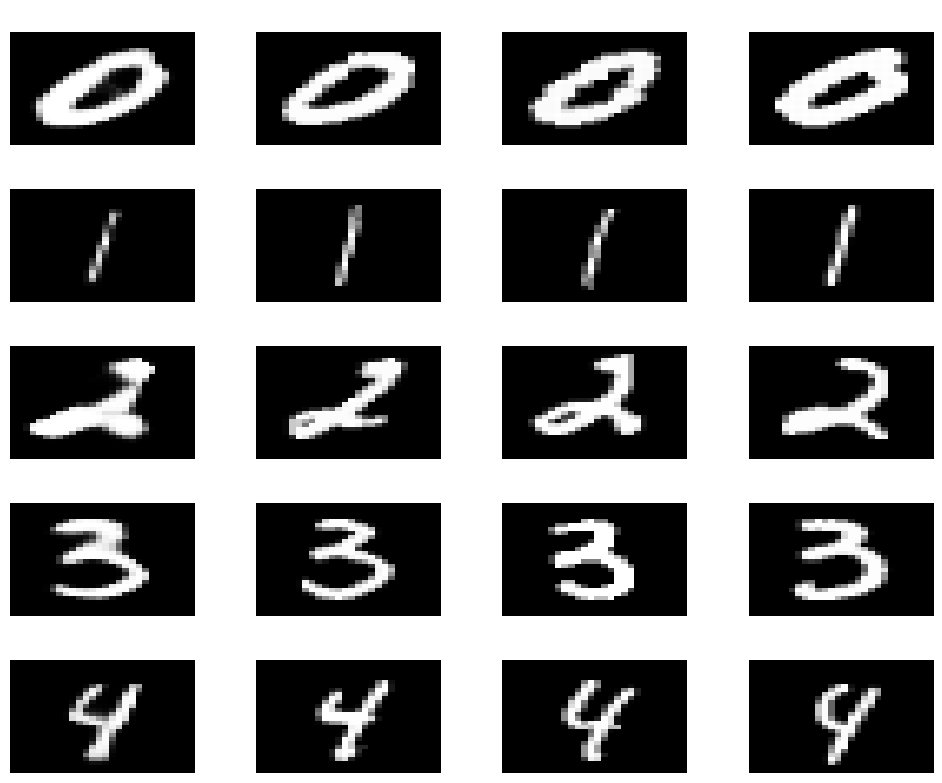
\includegraphics[width=0.9\linewidth]{./figures/nn-plot-final-0-4.png}
    \end{subfigure}%
    \begin{subfigure}{.5\linewidth}
      \centering
      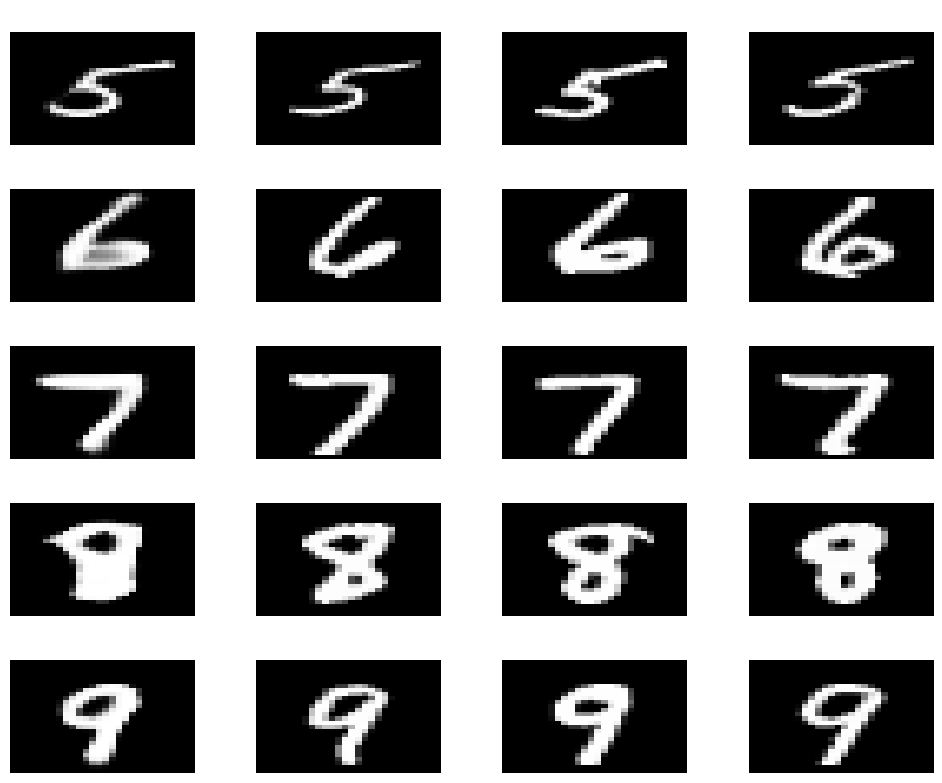
\includegraphics[width=0.9\linewidth]{./figures/nn-plot-final-5-9.png}
    \end{subfigure}

  \end{mdframed}
  \caption{\label{fig:mnist} Autoregressive Generation of Neural Field Weights for MNIST}
\end{figure}


\subsection*{Shapenet}

After the success on the 2D Task was verified, the approach was extended to 3D meshes from the Shapenet dataset. A subset of around 4k meshes from a single class, namely airplanes, was selected. The meshes were first converted to point clouds contained signed distance values for every point, as illustrated in Figure \ref{fig:airplane}. The point clouds were then used to train the neural fields. As with the MNIST Data a single sample from the dataset was firsttly overfitted and then used to initialize the other samples.








To handle the higher complexity of the 3D shapes in comparison to the 2D MNIST images, the neural network architecure of the implicit neural fields was extended. The hidden layers were increased to 32 neurons and an additional hidden layer was added. The input of x, y, z coordinates in again encoded using a sinusoidal positional encoding to 15 inputs. The output of the neural network is a single neuron with a tanh activation function.


\begin{figure}[H]
  \centering
  \includegraphics[width=\linewidth]{figures/sdf_plane.png}
  \caption{Example of a 3D Point Cloud from the Shapenet dataset.}
  \label{fig:airplane}
\end{figure}


% Flattening MLP-Sequence: Resulting in a sequence length of 3712.
% 1D Vector Quantization: Similar to the MNIST approach, the codebook was initialized using kMeans and optimized with L2 loss.
% Special Tokens: Introducing SOS-token and conditioning tokens to indicate the ShapeNet-NeF label.
% Mode Collapse
% During initial training, mode collapse was encountered, where only one mode of the true distribution was discovered. This was correlated with the conditioning weights of the neural field, resulting in stagnating cross-entropy. To address this:

\subsubsection*{Tokenization:}

To enable the generation of novel 3D shapes, a learned vocabulary was implemented. The MLP-weights were flattened to a sequence length of 3712 and a 1D Vector Quantization was applied. The codebook was initialized using kMeans and optimized with L2 loss. As with MNIST a SOS token was introduced to indicate to enable the generation of novel shapes.

\subsubsection*{Mode Collapse: }
During early training of the Transformer Model we experienced a model collapse where a local minimum to the Cross Entropy Loss formulation of the Transformer training was found in predicting only a single mode of the true distribution. Mode collapse is a phenomenon that is known to happen in GANs. The single mode that was generated by the model corresponded with the initializing weights of the neural field, resulting in stagnating cross-entropy. Additionally, the initialization neural field happened to be an airplane that is very similar to a larger portion of the airplanes in the dataset. Therefore, the initialization was changed to an airplane that belongs to a less frequent class in the dataset and additionally was pretrained using a L2-Regularization, to enforce that the neural field learns more diverse and better features.

\subsubsection*{Transformer}

Using the newly trained dataset of neural fields the transformer models were trained. Three different architectures of a decoder only GPT model were trained, whose implementation was inspired by NanoGPT \cite{Karpathy2022}. The model hyperparameters are shown in Table \ref{tab:architecture}.

\begin{table}[!htbp]
  \centering
  \begin{tabular}{l c c c}
    \toprule
    Parameter        & Small & Medium & Big  \\
    \midrule
    Embedding Size   & 256   & 384    & 512  \\
    Number of Heads  & 16    & 16     & 16   \\
    Number of Layers & 6     & 7      & 8    \\
    Vocabulary Size  & 128   & 128    & 128  \\
    Context Length   & 3712  & 3712   & 3712 \\
    \bottomrule
  \end{tabular}
  \caption{\label{tab:architecture} Transformer Architectures}
\end{table}


All models were trained for 1750 iterations, with an effective batch size of 32, and a learning rate of 3e-3. The models were trained using a cosine learning rate scheduler. The training and validation cross-entropy losses are shown in Figure \ref{fig:loss}.


\begin{figure}[!htbp]
  \centering
  \includegraphics[width=\linewidth]{figures/ce-loss-shapenet.png}
  \caption{Cross Entropy Loss during training}
  \label{fig:loss}
\end{figure}


\begin{figure*}[t]
  \centering
  \begin{subfigure}{.24\linewidth}
    \centering
    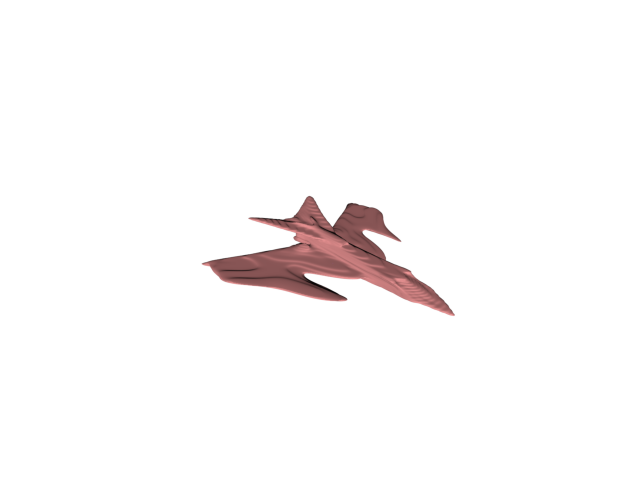
\includegraphics[width=\linewidth]{./figures/generation/0.png}
  \end{subfigure}
  \begin{subfigure}{.24\linewidth}
    \centering
    \includegraphics[width=\linewidth]{./figures/generation/1.png}
  \end{subfigure}
  \begin{subfigure}{.24\linewidth}
    \centering
    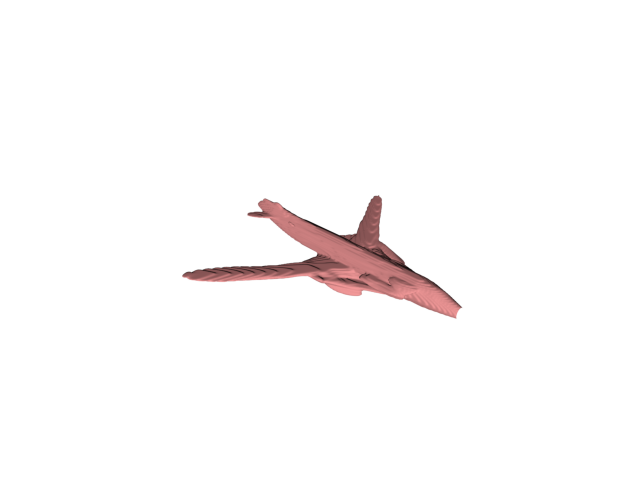
\includegraphics[width=\linewidth]{./figures/generation/2.png}
  \end{subfigure}
  \begin{subfigure}{.24\linewidth}
    \centering
    \includegraphics[width=\linewidth]{./figures/generation/3.png}
  \end{subfigure}
  \begin{subfigure}{.24\linewidth}
    \centering
    \includegraphics[width=\linewidth]{./figures/generation/4.png}
  \end{subfigure}
  \begin{subfigure}{.24\linewidth}
    \centering
    \includegraphics[width=\linewidth]{./figures/generation/5.png}
  \end{subfigure}
  \begin{subfigure}{.24\linewidth}
    \centering
    \includegraphics[width=\linewidth]{./figures/generation/6.png}
  \end{subfigure}
  \begin{subfigure}{.24\linewidth}
    \centering
    \includegraphics[width=\linewidth]{./figures/generation/7.png}
  \end{subfigure}

  \caption{\label{fig:generation} Autoregressive Generation of Neural Field Weights for Shapenet}

\end{figure*}


% L2-Regularization: Applied during training the conditioning neural field on unique planes in the dataset, which forced the NeF to learn more diverse and better features.
% Traditional Transformer
% The architecture for the traditional transformer in this context was to be refined in future iterations:

% Architecture: Details were to be finalized based on ongoing experiments and optimization.
% Results
% The metrics proposed by previous seminal works were adopted, specifically Minimum Matching Distance (MMD), Coverage (COV), and 1-Nearest-Neighbor Accuracy (1-NNA), to evaluate the quality of synthesized neural fields and compare them with established baselines.